\documentclass[12pt]{article}

\usepackage[utf8]{inputenc}
\usepackage[UTF8]{ctex}
\usepackage{sfmath}
\usepackage{amsmath}
\usepackage{graphics}
\usepackage{graphicx}
\usepackage{subfig}

\usepackage[super, sort&compress]{natbib}
\usepackage{hyperref}
\usepackage{url}

\usepackage{tikz}
\usetikzlibrary{shapes.geometric}
 
\usepackage{physics}

\usepackage{titling}
\pretitle{\begin{center}\Huge\bfseries}
\posttitle{\par\end{center}\vspace{0.5cm}}
\preauthor{\begin{center}\large}
\postauthor{\par\end{center}}
\predate{\begin{center}\large}
\postdate{\par\end{center}}

\usepackage{geometry}
\geometry{a4paper, margin=1in}

\title{
    Mechatronics and Making \\
    Mid-Term Project Report \\
    Exoskeleton Robotic Hand With Wolf Claw Mechanism
}


\author{
    \begin{align*}
        \text{Bryan Li}\ &-  \text{SN 25003743} \\
        \text{Yan Pei Zhu}\ &-  \text{SN 25103352}\\
        \text{Nolan Yu}\ &-  \text{SN 25113715}
    \end{align*}
}

\date{October 31, 2025}

\setlength{\parindent}{0pt}
\setlength{\parskip}{1em}


\begin{document}

\begin{titlepage}
	\maketitle
\end{titlepage}

\tableofcontents

\pagebreak

\section{Introduction}
\subsection{Project Objectives and Description}
\subsection{Similar Mechanisms}
\subsection{Industrial Applications}

\pagebreak

\section{Mechanical and Mechanism Analysis}

\subsection{Drive Method and Transmission}
This robotic hand exoskeleton uses an acceleration-based machinery system.
Therefore, the movements of the finger will be amplified by this mechanism.

This mechanism can do that through a planetary gear mechanism,
whereas a belt system and a string transmission system are also needed.

Details of the transmission process shows below:

\begin{center}
	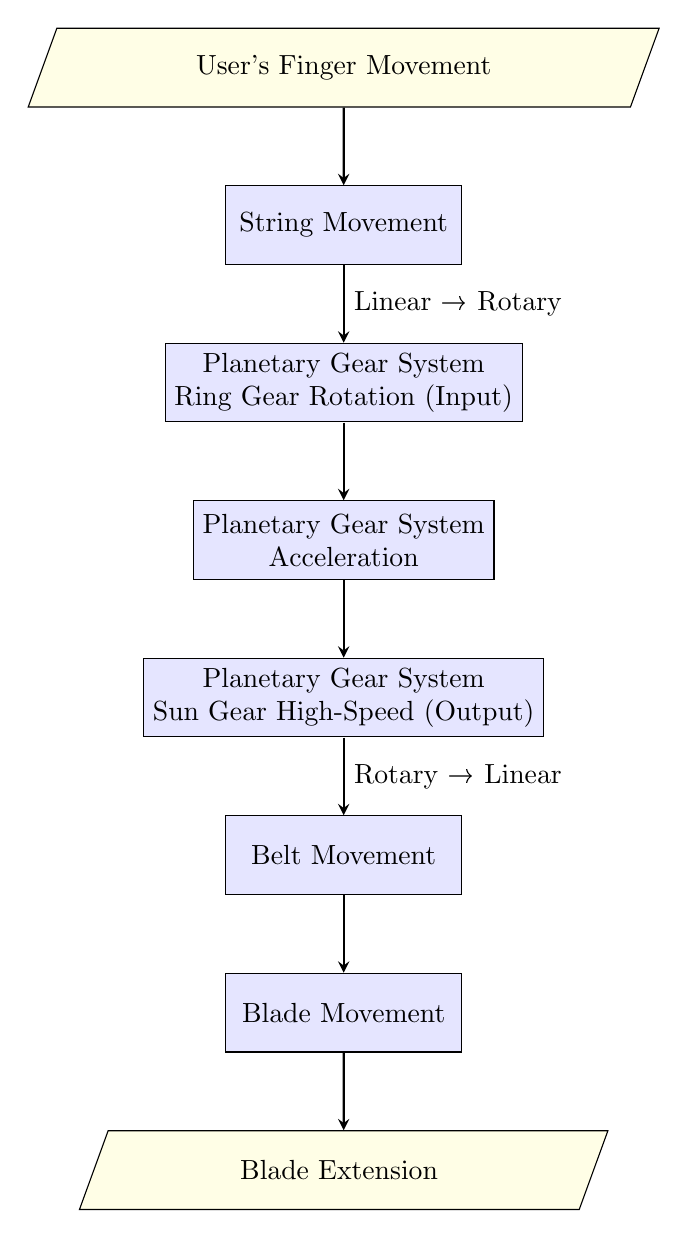
\begin{tikzpicture}[scale=0.8]

		% Define styles
		\tikzstyle{process} = [
		rectangle, minimum width=3cm, minimum height=1cm,
		text centered, draw=black, fill=blue!10, align=center]
		\tikzstyle{io} = [
		trapezium, trapezium left angle=70,
		trapezium right angle=110, minimum width=3cm,
		minimum height=1cm, text centered, draw=black,
		fill=yellow!10, align=center]
		\tikzstyle{arrow} = [thick,->,>=stealth]

		% Nodes
		\node (start) [io] {User's Finger Movement};

		\node (tendon) [process, below of=start, yshift=-1cm] {String Movement};

		\node (ring) [process, below of=tendon, yshift=-1cm] {
			Planetary Gear System \\
			Ring Gear Rotation (Input)
		};

		\node (planetary) [process, below of=ring, yshift=-1cm] {
			Planetary Gear System \\
			Acceleration
		};

		\node (sun) [process, below of=planetary, yshift=-1cm] {
			Planetary Gear System \\
			Sun Gear High-Speed (Output)
		};

		\node (pulley) [process, below of=sun, yshift=-1cm] {Belt Movement};

		\node (belt) [process, below of=pulley, yshift=-1cm] {Blade Movement};

		\node (blade) [io, below of=belt, yshift=-1cm] {
			Blade Extension
		};


		% Arrows
		\draw [arrow] (start) -- (tendon);
		\draw [arrow] (tendon) -- node[right] {Linear → Rotary} (ring);
		\draw [arrow] (ring) -- (planetary);
		\draw [arrow] (planetary) -- (sun);
		\draw [arrow] (sun) -- node[right] {Rotary → Linear}(pulley);
		\draw [arrow] (pulley) -- (belt);
		\draw [arrow] (belt) -- (blade);
	\end{tikzpicture}
\end{center}

\pagebreak

\subsection{Hand Exoskeleton Mechanisms}
\subsubsection{Hand Structure}
根据Heo等人(2012)的综述,人手包含19块骨骼和14个关节(不包括腕骨)。手指关节主要包括:

掌指关节(MCP):具有2个自由度(屈曲/伸展、外展/内收)

近端指间关节(PIP) 和 远端指间关节(DIP):各具1个自由度(屈曲/伸展)

拇指 的腕掌关节(CMC)为鞍状关节,具有2个自由度,赋予其更大的灵活性。

在休息姿态下,MCP关节屈曲约45°,PIP屈曲30–45°,DIP屈曲10–20°。这些数据对于设计外骨骼时的运动范围和安全性至关重要。

\subsection{Wolf Claw Mechanism Comparison}
\subsubsection{Version 1: Planetary Gear}
\subsubsection{Version 2: Compound Gear Train}


\pagebreak

\section{Mathematical Modelling and Analysis}
\subsection{Fingers and Wrist Modelling}
\textbf{User's Input (Finger Movement)}

The linear movement of the string that is deployed over the finger is created by the finger's flexion.

Figure~\ref{fig:mid_finger} has two sub-figures:
Figure~\ref{fig:mid_finger_curved} describes the details and data when finger curved,
Figure~\ref{fig:mid_finger_extended} describes the details and data when finger extended.


\begin{figure}[htbp]
	\centering
	\subfloat[mid-finger curved\label{fig:mid_finger_curved}]{
		\includegraphics[width=0.4\textwidth]{imgs/mid_fig_curved.PNG}
	}
	\hfill
	\subfloat[mid-finger extended\label{fig:mid_finger_extended}]{
		\includegraphics[width=0.5\textwidth]{imgs/mid_fig_extend.PNG}
	}
	\caption{mid-finger exoskeleton design}\label{fig:mid_finger}
\end{figure}

Total displacement of the string overhead by calculation:\cite{bryan}

\begin{align*}
	\Delta L             & = L_{DIP} + L_{PIP} + L_{MCP}, \quad \text{where}     \\
	L_{DIP}              & = 11 \times \frac{45}{360} \times 2\pi \approx 8.64,  \\
	L_{PIP}              & = 11 \times \frac{60}{360} \times 2\pi \approx 11.52, \\
	L_{MCP}              & = (25 - 11) \times \frac{85}{360} \times 2\pi \approx 20.77 \\
	\Rightarrow \Delta L & \approx 8.64 + 11.52 + 20.77 = \boxed{40.93\text{mm}} \\
\end{align*}
\subsection{Wolf Claw Mechanism \- Version 1: Planetary Gear}
\subsection{Wolf Claw Mechanism \- Version 2: Compound Gear Train}

\pagebreak
\section{Conclusion and Future Work}

\pagebreak

\bibliographystyle{plain}
\bibliography{references}

\end{document}
